
\documentclass{article}

\usepackage{graphviz}
\usepackage{url}
\usepackage{hyperref}
\usepackage{fullpage}
\usepackage{parskip}
\usepackage{fancyvrb}
\usepackage{amsmath}
\usepackage[section]{placeins}
\usepackage{tikz-timing}

\usepackage{listings}
\lstset{numbers=left,
		basicstyle=\footnotesize,
		captionpos=b,
		xleftmargin=0.3in}

\usepackage[backend=biber,autocite=footnote,
	            bibstyle=authortitle,citestyle=verbose-inote]{biblatex}
\addbibresource{main.bib}
\setlength\bibitemsep{1em}

\usepackage[xindy,toc,nonumberlist]{glossaries}
\makeglossaries
\renewcommand*{\glspostdescription}{}

\providecommand{\e}[1]{\ensuremath{\times 10^{#1}}}

\VerbatimFootnotes

\raggedright

\begin{document}

% {{{ glossary entries

\newglossaryentry{SPI}
{
	name={SPI},
	description={Serial peripheral interface}.
}

\newglossaryentry{MOSI}
{
	name={MOSI},
	description={(SPI) master out slave in}.
}

\newglossaryentry{MISO}
{
	name={MOSI},
	description={(SPI) master in slave out}.
}

\newglossaryentry{GPIO}
{
	name={GPIO},
	description={General purpose input/output}.
}

\newglossaryentry{FIFO}
{
	name={FIFO},
	description={First in first out}.
}


% }}}

% {{{ title page
\vspace*{1.0in}

\centerline{\Large \textbf{SprinklerPI}}
\centerline{(Design)}

\vspace{0.5in}

\begin{center}
\begin{tabular}{c}
Jeremiah Mahler \\
EECE 490B, CSU Chico \\
\today
\end{tabular}
\end{center}

\thispagestyle{empty}

\vfill

\pagebreak
% }}}

\nocite{rasberrypi}
\thispagestyle{empty}
\tableofcontents

% {{{ Architectural Design
\clearpage
\section{Architectural Design}

At the highest level the SprinklerPI system creates a web interface
for controlling sprinkler valves.
Figure \ref{fig:archoview} gives an overview.

\begin{figure}[h!]
\begin{center}
\includegraphics[scale=0.5]{dia/architectural_overview}
\end{center}
\caption{Overview of SprinklerPI in system.}
\label{fig:archoview}
\end{figure}

There are many subcomponents of the SprinklerPI system.
The power supply must take 110 volts AC from a residential outlet
The power supply must take 110 volts AC from a residential outlet
and convert it to 24 volts AC and 5 volts DC.
The 24 volts AC is needed to drive the sprinkler valves.
The 5 volts DC is needed for the Linux computer and the digital logic (control).
The digital logic (control) must take accept a command over SPI
and turn on one of the sprinkler valves or turn them all off.
The driver must take a digital logic input and drive the appropriate
sprinkler valve using 24 volts AC.
The web based user interface must allow the timer schedules to be
set and for the valves to be manually operated.
Figure \ref{fig:spioview} gives an overview of the major components
inside the SprinklerPI system.

\begin{figure}[h!]
\begin{center}
\includegraphics[scale=0.47]{dia/sprinklerpi_overview}
\end{center}
\caption{Overview of main components inside the SprinklerPI system.}
\label{fig:spioview}
\end{figure}

% }}}

% {{{ Hardware Design
\clearpage
\section{Hardware Design}
\label{sec:hardware}

There are three main hardware components in this system.
First is the power supply.
It takes 110 volts AC and outputs both 5 volts DC and 24 volts AC.
The sprinkler valves require 24 volts AC.
The Linux computer and digital logic require 5 volts DC.
Second is the Linux computer which is a standard RasberryPI model B.
And third is the Control Driver which contains all the
circuitry needed to accept commands using SPI from the RasberryPI
and to drive up to eight individual sprinkler valves.
Additional Control Drivers can be added to drive additional sprinkler
valves.
Each individual Control Driver supports eight valves.
To keep the system modular each of these modules will be on a
separate PCB.
Figure \ref{fig:hwoview} gives an overview of the hardware in the system.

\begin{figure}[h!]
\begin{center}
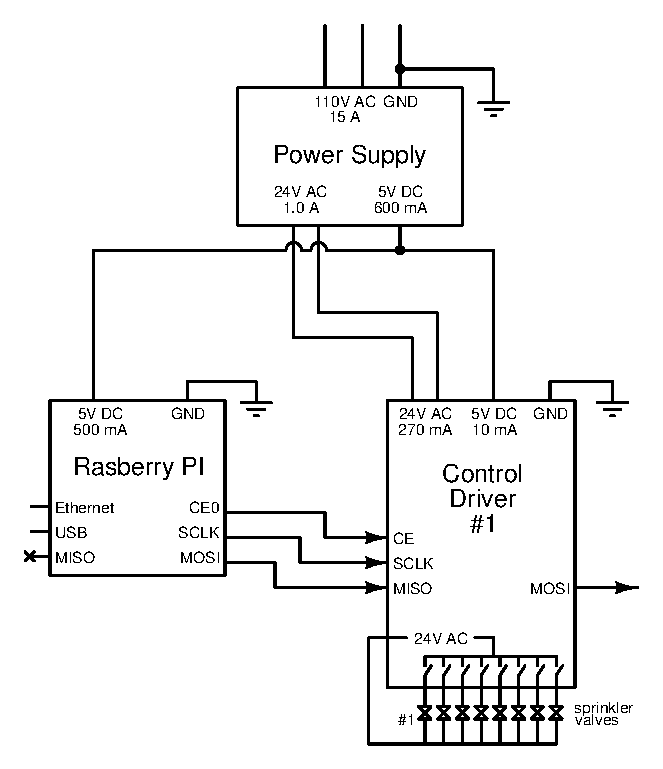
\includegraphics[scale=0.9]{xcircuit/hardware_overview}
\end{center}
\caption{Overview of hardware in system.
Only one control/driver is shown, 
additional control/drivers can be added up to a maximum of three.
Expansion is limited by the power supply.}
\label{fig:hwoview}
\end{figure}

% {{{ State Flow Diagrams
\subsection{State Flow Diagrams}

The primary module of interest with regard to state flow is
the Control Driver (Figure \ref{fig:hwoview}).
It controls the sprinkler valves based on commands it receives
from the Linux computer (RasberryPI) over SPI.

The Control Driver is always either driving one of the eight valves
or has all of the valves off.
The only time this changes is when a new command is sent.

During power on all the valves must remain in the off state.
If this were not required, and the system entered some random
state during power on, a valve could be inadvertently turned on.
And since there is no watchdog mechanism this valve would remain
on until the next command was received.
Figure \ref{fig:hwstate} shows the state machine of the
Control Driver circuitry in hardware.

\begin{figure}[h!]
\centering
\includegraphics[scale=0.48]{dia/hardware_state}
\caption{State diagram of hardware control circuitry.
During power on it is important that the valves remain off.
In the idle state it waits for a command to turn on a valve or
turn off all valves.}\label{fig:hwstate}
\end{figure}

The hardware state is determined by the control circuitry
described in Section \ref{sec:control}.

% }}}

% {{{ Schematics
\clearpage
\FloatBarrier
\subsection{Schematics}

% {{{ Control
\FloatBarrier
\subsubsection{Control}
\label{sec:control}

Before a sprinkler valve can be driven some control logic is necessary
between the RasberryPI and the driver (Section \ref{sec:driver}).
Most residential sprinkler systems are capable of driving eight circuits.
And only one of these circuits is active at any one time
\footnote{If multiple circuits were active this could lower the
water pressure resulting in inconsistent watering amounts.}.
This controller uses the same design.

The RasberryPI has enough GPIO pins to control each valve independently.
But doing this would be a waste.
Future expansion to a large number of circuits would be limited.
Also the time requirements for are very generous.
Being able to switch valves at 1 Hz is more than adequate.

Instead of using individual GPIO pins, the four SPI pins provided by
the SPI are used.
This design sends 8-bits for each message (Figure \ref{fig:spi}).
But only three bits are used to address each valve ($2^3 = 8$).
If the design was expanded to use the available bits
it could address 128 valves ($2^7 = 128$).
The single enable bit was chosen to simplify the circuitry.
However it does reduce the maximum number of addresses by one bit.

{
\renewcommand*\arraystretch{1.5}
\begin{figure}[hbp]

\centering
\begin{tabular}{l r l r l r }
7 & 4 & 3 & 1 & \multicolumn{2}{c}{0} \\
\hline
\multicolumn{2}{|c|}{\hspace*{6mm} unused \hspace*{6mm}} &
\multicolumn{2}{|c|}{\hspace*{4mm} valve \hspace*{4mm}} &
\multicolumn{2}{|c|}{\hspace*{1mm} en\_n \hspace*{1mm}} \\
\hline
\end{tabular}

\caption{SPI message format.}
\label{fig:spi}
\end{figure}
}

Translating a 8-bit message received over SPI to signal turn on
a sprinkler valve requires a small amount of discrete logic.
A shift register is needed to take the bits as inputs.
A decoder is needed to convert shifted in number to a single
bit output.
In this case a 74HC238 3-8 decoder is used since it provides non-inverting
outputs.
An output high will turn on a valve.
Figure \ref{fig:control} shows the control schematic.

\begin{figure}[hbp]
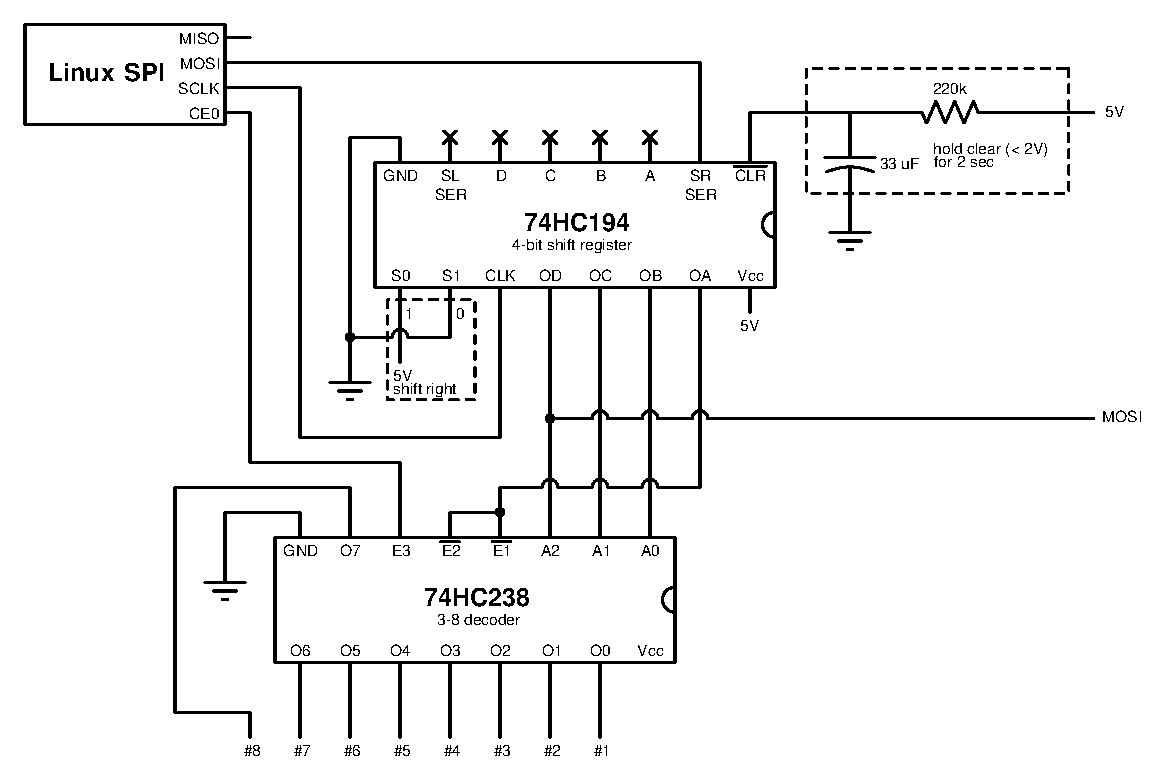
\includegraphics[scale=0.85]{xcircuit/control}
\caption{Sprinkler valve control logic.
Sprinkler valve number is input using SPI from the RasberryPI in
to the shift register.  The number is decoded and inverted to produce
a single high signal for one valve.
All outputs are disabled when OA is clear.}\label{fig:control}
\end{figure}

On power up it is important that the valves remain off.
However the shift register chip (74HC194) does not guarantee
the output state during power up.
To resolve this issue a simple RC circuit is used to to hold the
chip in the clear state for several seconds after power
on (Figure \ref{fig:control}).

% }}}

% {{{ Driver
\FloatBarrier
\subsubsection{Driver}
\label{sec:driver}

The control circuit (Section \ref{sec:control}) provides a digital
output signal in the range of 0 to 5 volts DC.
This signal is inadequate for driving the sprinkler valve which
requires 24 volts AC.
The driver circuit discussed here is used to apply 24 volts AC
signal when triggered by a 5 volts DC signal.

\begin{figure}[hbp]
\centering
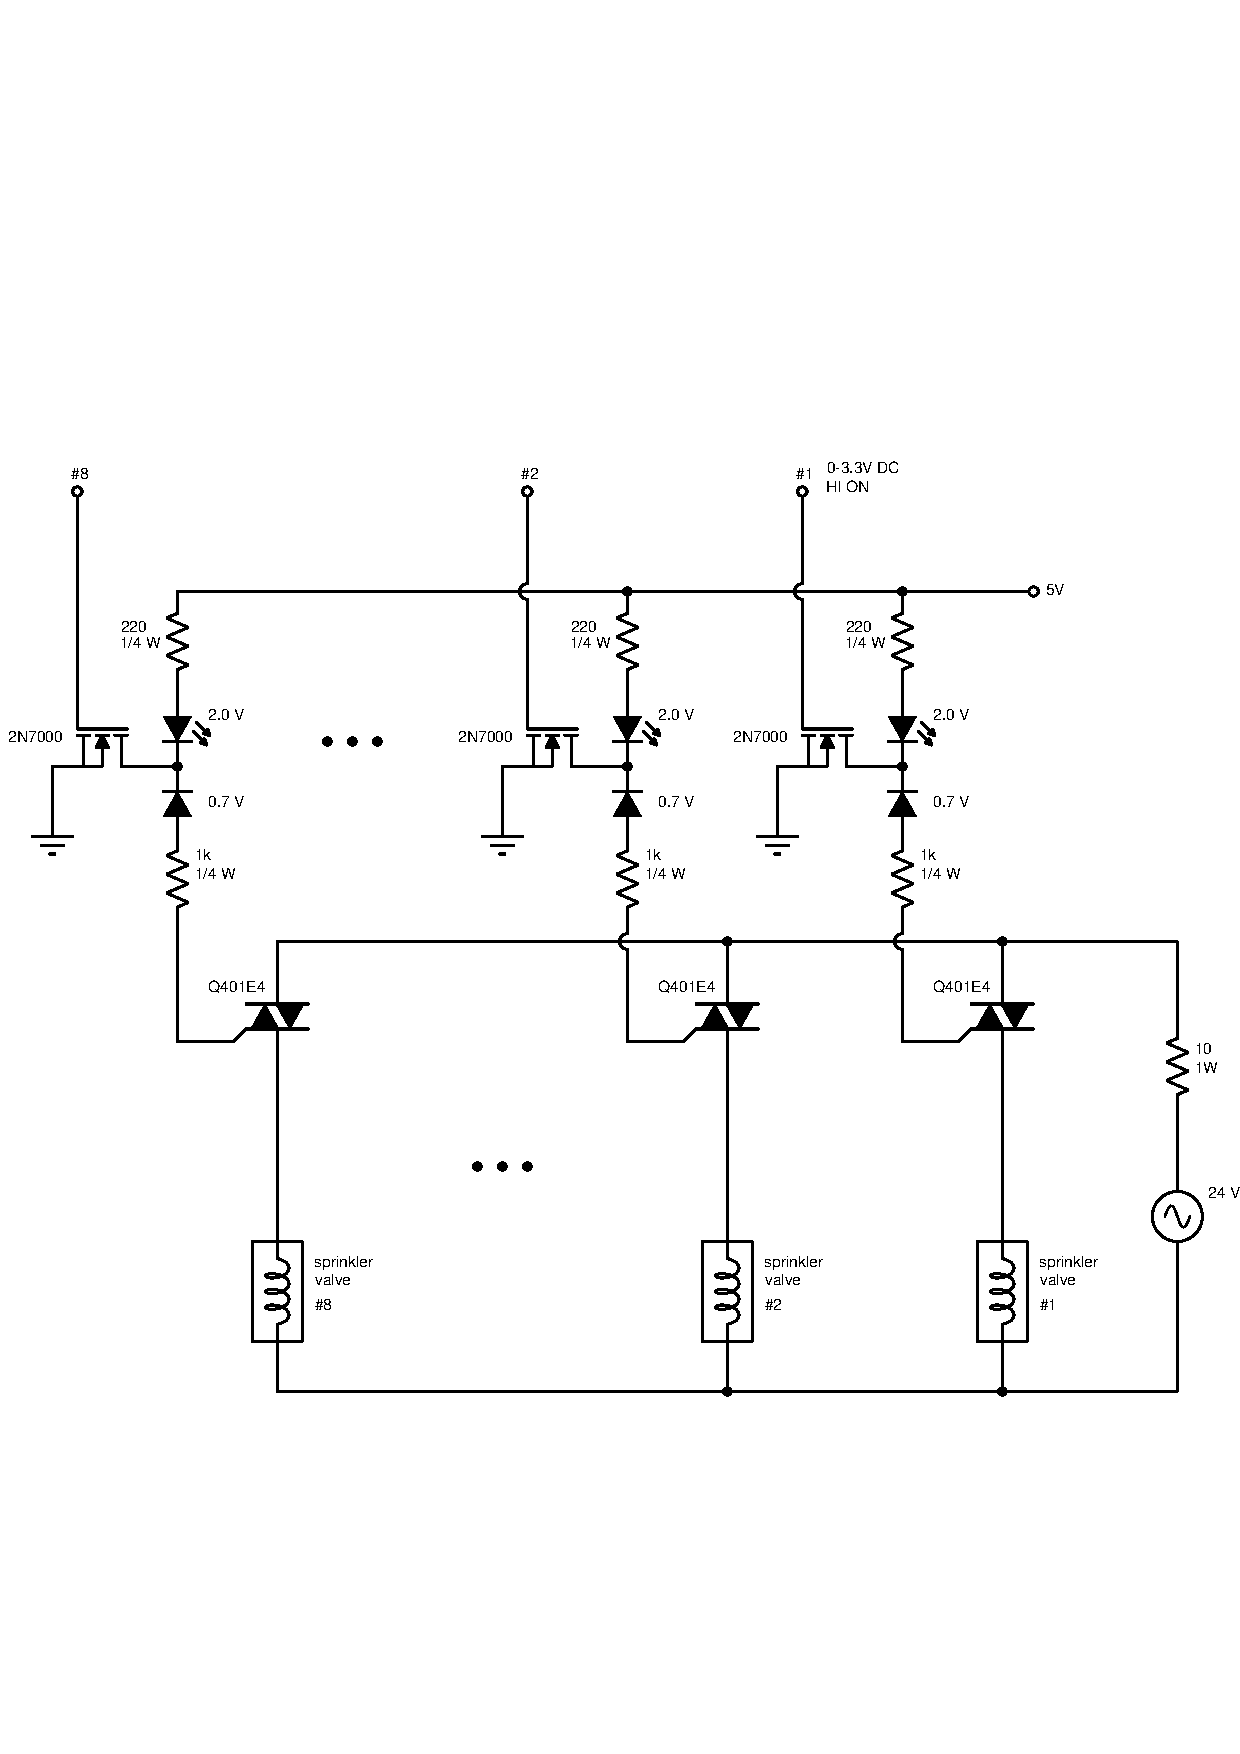
\includegraphics[scale=0.7]{xcircuit/driver_mult}
\caption{Sprinkler valve driver circuits.
Not all branches are shown since they are identical.
LEDs are used to indicate when the valve is on/off.
It is assumed that only one valve will be on at a time.}\label{fig:driver}
\end{figure}

To turn the sprinkler valves on requires 24 VAC at approximately 270 mA.
If it is assumed that during steady state both the solenoid
and the triac have negligible resistance (Figure \ref{fig:driver}),
a 10 $\Omega$ resistor can be used to limit the current to 270 mA.
At 1 watt the resistor supports the worst case amperage with a margin
over 10\%.

\begin{align*}
	P &= I^2 R \\
	  &= (270\e{-3})^2 \cdot 10 \\
	  &= 0.729 \quad \text{[W]}
\end{align*}

The control signal to the triac (Q401E4) is very sensitive.
The tinyest current will cause it to conduct.
If it is driven by a 0-5V signal it will conduct not only
with a 5V signal but also with 0V signal.
To overcome this issue a diode was used to ensure no current
flows when it is reverse biased.
The FET (2N7000) is used to switch the triac while it also
serves to limit the control current of a 0-5 volt signal
to less than 0.5 mA.
This places the control current well within the limits
of CMOS logic as required by the control chips (Section \ref{sec:control}).

% }}}

% {{{ Power Supply
\subsubsection{Power Supply}
\label{sec:power}

The power supply must provide two different voltages: 24 volts AC and
5 volts DC.
The sprinkler valves require 24 volts AC at 270 mA.
The Linux computer and other digital logic require 5 volts DC with a
maximum draw of 600 mA
\footnote{The current draw of the RasberryPI was determined
experimentally to be approximately 500 mA.}.
These voltages must be created from a 110 volt AC input.

The 24 volts AC can be achieved using a split pole transformer
with two 12 volt AC outputs.
By bridging the center of these two 12 volt AC outputs
a combined 24 volt AC output is available.

A switching voltage regulator, the MC34063A, was chosen for
the 5 volt supply.
It has a greater efficiency than a linear regulator such as
the LM7805.

The circuit which achieves all of these design requirements is
shown in Figure \ref{fig:power}.

\begin{figure}[hbp]
\centering
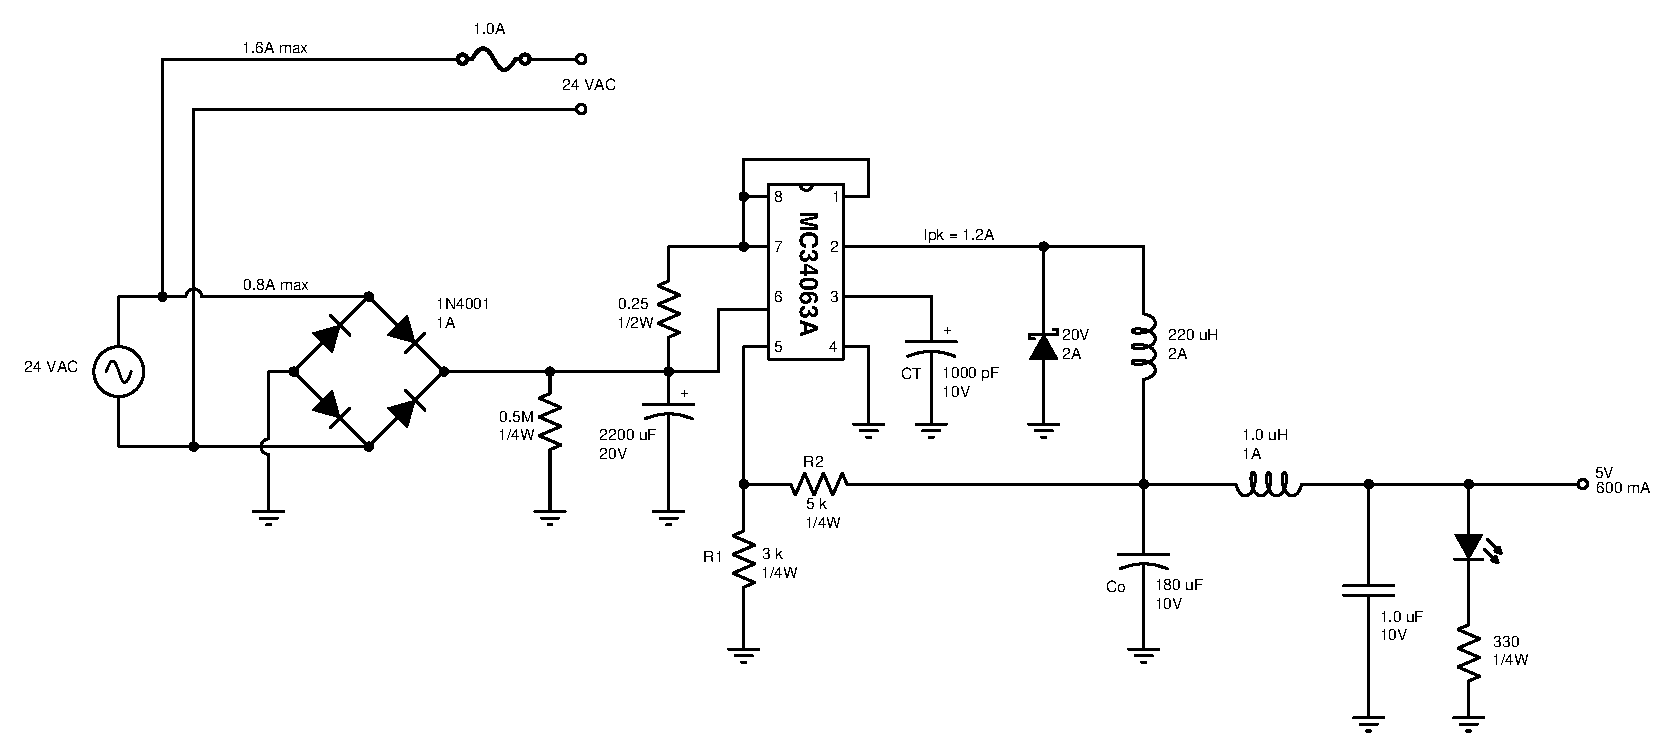
\includegraphics[angle=90,scale=0.70]{xcircuit/power_supply}
\caption{Power supply circuit. A 24 volt AC and 5 volt DC output are
provided.  The 5 volt DC is provided by the MC340363A switching
regulator.}\label{fig:power}
\end{figure}

% }}}

% }}}

% {{{ Timing Diagrams
\FloatBarrier
\subsection{Timing Diagrams}

Figure \ref{fig:timing} is a diagram of a message being sent
using SPI from the Linux computer to the control module.
Refer to Section \ref{sec:control} for a description of
the meaning of these messages.

\begin{figure}[h!]
\begin{center}
\begin{tikztimingtable}
	[xscale=2.0, yscale=2.0]
	CE	 & {1H} 1{C} {12L} 1{C} {1H} \\
	SCLK & {1H} 14{C} {1H} \\
	MOSI & 10L 1{C} 1{H} 1{C} 3L \\
	MISO & 16L \\
\end{tikztimingtable}
\end{center}
\caption{Timing diagram of a message sent using SPI from
the RasberryPI to a control module.
A value from MOSI is latched on the rising edge of SCLK.
In this case the value 2 is transferred.}
\label{fig:timing}
\end{figure}
% }}}

% {{{ Theory of Operation
\FloatBarrier
\subsection{Theory of Operation}

% describe external interface

The operation of the hardware as a whole provides the ability to
turn a valve on or to turn them all off.
One valve can be on at a time for a single Control Driver module.
Commands are written over SPI from the Linux computer (RasberryPI).

The user interface, described in Section \ref{sec:swdesign}, will
establish a friendly user interface on top of this simple hardware
interface.

% }}}

% }}}

% {{{ Software Design
\FloatBarrier
\section{Software Design}
\label{sec:swdesign}

The software creates a user interface for controlling
and scheduling the sprinkler valves.
Figure \ref{fig:swoview} gives an overview of the system.

\begin{figure}[htbp!]
\begin{center}
\includegraphics[scale=0.45]{dia/software_overview}
\end{center}
\caption{Overview of software in the sprinkler control system.
The web server (www) communicates with the queue daemon
using a set of files.
The queue daemon monitors the queue and controls the valves accordingly.
The timer daemon adds jobs to the queue according to the timer schedule.}
\label{fig:swoview}
\end{figure}

\FloatBarrier
\subsection{File System}

Interprocess communication between the queue daemon, the web server
and the timer daemon is accomplished using files.
The following is a listing of the files that are present.

\begin{verbatim}
sprinklerpi/
  queue
  valve
  clear
  log
  timer/
    valve1
     ...
    valve8
\end{verbatim}

\begin{itemize}
    \item \verb+queue+ - Queue of jobs to execute.
    \item \verb+valve+ - Current valve number that is running.
        Zero if none are running.
    \item \verb+clear+ - When true the queue daemon clears the queue.
        It is reset to false after queue is cleared.
    \item \verb+log+ - Log of operations queue-daemon has performed.
    \item \verb+timer/valve*+ - Schedule of when each valve should run.
\end{itemize}

\FloatBarrier
\subsection{Queue Daemon}

The queue daemon monitors the queue file and executes the command.
An example command might be ``run valve 3 for 5 minutes''.
Figure \ref{fig:queue-daemon} gives a flow chart of its operation.

\begin{figure}[htbp!]
\begin{center}
\includegraphics[scale=0.45]{dia/queue-daemon}
\end{center}
\caption{Flow chart of the queue daemon operation.}
\label{fig:queue-daemon}
\end{figure}

% TODO - abort operation?

\clearpage
\FloatBarrier
\subsection{Timer Daemon}

The timer daemon monitors the valve schedule and adds jobs
to the queue when they are ready to be run.
Figure \ref{fig:timer-daemon} gives a flowchart of its operation.

\begin{figure}[htbp!]
\begin{center}
\includegraphics[scale=0.45]{dia/timer-daemon}
\end{center}
\caption{Flow chart of the timer daemon operation.}
\label{fig:timer-daemon}
\end{figure}

% }}}

% {{{ Future Directions
\section{Future Directions}

\subsection{Automated Hardware Testing}

Currently the operation of the system can be manually
verified by a user.  There are LED indicators to show
when a valve is on/off.  And programs can be written
to operate all the valves.
It can also be verified by a user that the sprinkler
valves operate when connected to an actual sprinkler
system.
However this process is far too slow and costly for
testing this system if it was manufactured.

One solution is to create an additional module which
can place a load on the driver circuit for each of
the eight valves.
And by measuring the voltage/current it can be determined
if the correct circuit is being actuated and if
its rated current is being drawn.

And programs can be written to control the system and
verify its operation using this test module.
The entire system could be tested and verified in a
few minutes.

\begin{figure}[htbp!]
\begin{center}
\includegraphics[scale=0.45]{dia/tester}
\end{center}
\caption{Automated testing system.
The tester is connected in place of the actual sprinkler valves.}
\label{fig:tester}
\end{figure}

\subsection{i2c Bus}

The SPI bus will become cumbersome to use with many
controllers.
In a daisy chain configuration each controller requires
eight bits.
As an example, with ten controllers an eighty bit command
would have to be sent.

A more capable bus such as i2c, LIN or CAN might be a good alternative.

\subsection{Internet of Things}

The Internet of Things\autocite{wiki:iot} is a term used to describe
the many Internet accessible devices which becoming more prevalent.
In particular, devices that uniquely identify themselves using RFID
tags or by some other means.
Most often these are household devices.

However the Internet of Things is still in its infancy.
Specifications are being written but it is still not precisely
clear exactly what constitutes an Internet of Things device.

The SprinklerPI is Internet accessible which is an obvious
characteristic of Internet of Things.
And it is likely that when a specific protocol or interface becomes
established the SprinklerPI system could be made to support it.

Currently the SprinklerPI system is manually configured and a known
network address is required to access it.
Internet of Things devices are typically auto-identified and easier
to setup.
It may be worthwhile to try and make the SprinklerPI system easier
to configure and setup in this way.
Perhaps a barcode on the device which maps to a url.
Then a phone could easily reach the interface for that device.

More research is needed to see what characteristics of Internet of Things
devices can be used.
Or even whether one of the burgeoning protocols could be implemented.

% }}}

\pagebreak
\glsaddall
\printglossaries

% References
\clearpage
\printbibliography[heading=bibintoc]

\end{document}

